\subsection{Doppler-Effekt}
    \subsubsection{Ohne relativistischen Effekt (Bsp. Schall)}
    Wenn Empfänger sich auf Sender zubewegt:
    \mathbox{f' = f_0 (1 + \frac{v}{c})}

    \begin{minipage}{0.22\linewidth}
            \mathbox{\lambda_0 = \frac{c}{f_0}}
    \end{minipage}
    \begin{minipage}{0.70\linewidth}
        \begin{center}
            \begin{empheq}[box=\fbox]{align*}
                \text{Schallgeschwindigkeit: } &= 340 \frac{m}{s}\\
                \text{Lichtgeschwindigkeit: } &= 3 \cdot 10^8 \frac{m}{s}
            \end{empheq}
        \end{center}
    \end{minipage}
    \vspace{2mm}


    \begin{minipage}{0.49\linewidth}
        \textbf{Empfänger auf Sender:}\\
        \begin{center}
            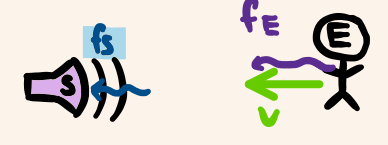
\includegraphics[width = 0.49\linewidth]{src/images/Doppler_E_zu_S.png}
        \end{center}
    \end{minipage}
    \begin{minipage}{0.49\linewidth}
        \begin{center}
            \begin{empheq}[box=\fbox]{align*}
                f' = f_0 (1 + \frac{v}{c})
            \end{empheq}
        \end{center}
    \end{minipage}
    \vspace{2mm}

    \begin{minipage}{0.49\linewidth}
        \textbf{Empfänger von Sender weg:}\\
        \begin{center}
            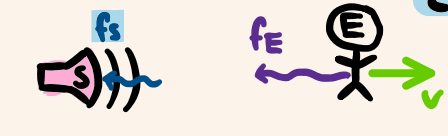
\includegraphics[width = 0.49\linewidth]{src/images/Doppler_E_weg_S.png}
        \end{center}
    \end{minipage}
    \begin{minipage}{0.49\linewidth}
        \begin{center}
            \begin{empheq}[box=\fbox]{align*}
                f' = f_0 (1 - \frac{v}{c})
            \end{empheq}
        \end{center}
    \end{minipage}
    \vspace{2mm}


    \begin{minipage}{0.49\linewidth}
        \textbf{Sender auf Empfänger:}\\
        \begin{center}
            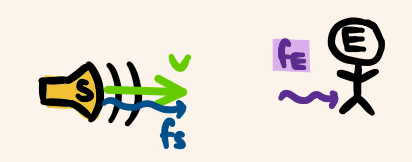
\includegraphics[width = 0.49\linewidth]{src/images/Doppler_S_zu_E.png}
        \end{center}
    \end{minipage}
    \begin{minipage}{0.49\linewidth}
        \begin{center}
            \begin{empheq}[box=\fbox]{align*}
                f' = f_0 \frac{1}{1 - \frac{v}{c}}
            \end{empheq}
        \end{center}
    \end{minipage}
    \vspace{2mm}


    \begin{minipage}{0.49\linewidth}
        \textbf{Sender von Empfänger weg:}\\
        \begin{center}
            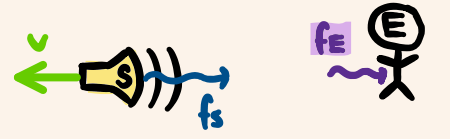
\includegraphics[width = 0.49\linewidth]{src/images/Doppler_S_weg_E.png}
        \end{center}
    \end{minipage}
    \begin{minipage}{0.49\linewidth}
        \begin{center}
            \begin{empheq}[box=\fbox]{align*}
                f' = f_0 \frac{1}{1 + \frac{v}{c}}
            \end{empheq}
        \end{center}
    \end{minipage}
    \vspace{2mm}

    \begin{flushleft}
    Für $v << c$ gilt, dass es nicht drauf ankommt ob Sender oder Empfänger sich in Ruhe befindet.

    \subsubsection{Mit relativistischem Effekt ($v \rightarrow c_0$)}
    $\beta = \frac{v}{c}$
    \vspace{2mm}

    
    
        \textbf{Quelle und Empfänger entfernen sich (Redshift):}\\
        \mathbox{f' = f_0 \sqrt{\frac{1 - \beta}{1 + \beta}}}

        \textbf{Quelle und Empfänger nähern sich (Blueshift):}\\
        \mathbox{f' = f_0 \sqrt{\frac{1 + \beta}{1 - \beta}}}
    \end{flushleft}\


    